\chapter{Конструкторская часть}

В данном разделе будут определены требования к программному обеспечению и приведены схемы алгоритма полного перебора и муравьиного алгоритма для решения задачи коммивояжера.

\section{Требования к программному обеспечению}

К разрабатываемой программе предъявлен ряд требований:

\textbf{Входные данные:} Взвешенный неориентированный граф, заданный матрицей стоимостей.

\textbf{Выходные данные:} Оптимальный гамильтонов цикл и субоптимальный гамильтонов цикл при использовании алгоритма полного перебора и муравьиного алгоритма соответственно.

\section{Схемы алгоритмов}

На рисунках~\ref{fig:brute_force}~---~\ref{fig:ant} представлены схема алгоритма полного перебора и схема муравьиного алгоритма.

\begin{figure}[H]
    \centering
    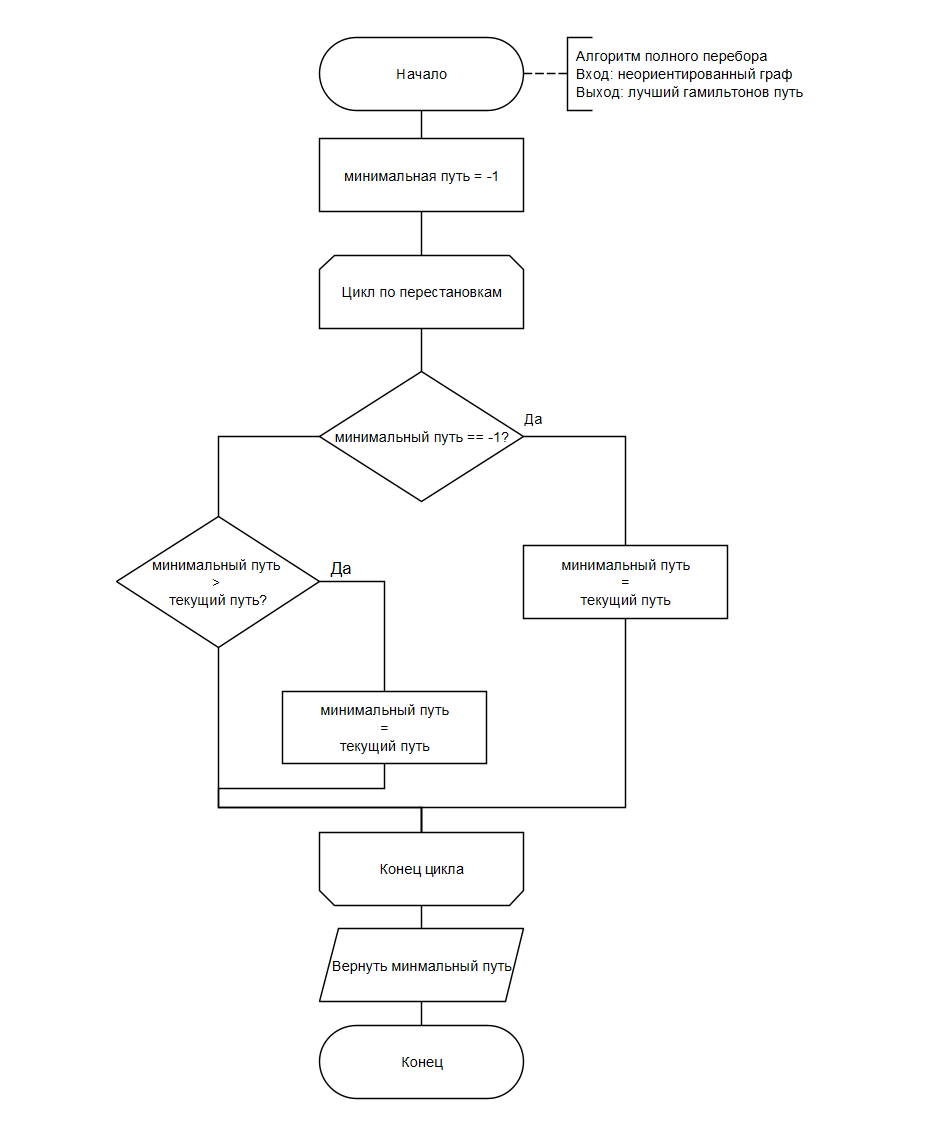
\includegraphics[width=1\linewidth]{images/schemes/brute_force.png}
    \caption{Схема алгоритма полного перебора}
    \label{fig:brute_force}
\end{figure}

\begin{figure}[h]
    \centering
    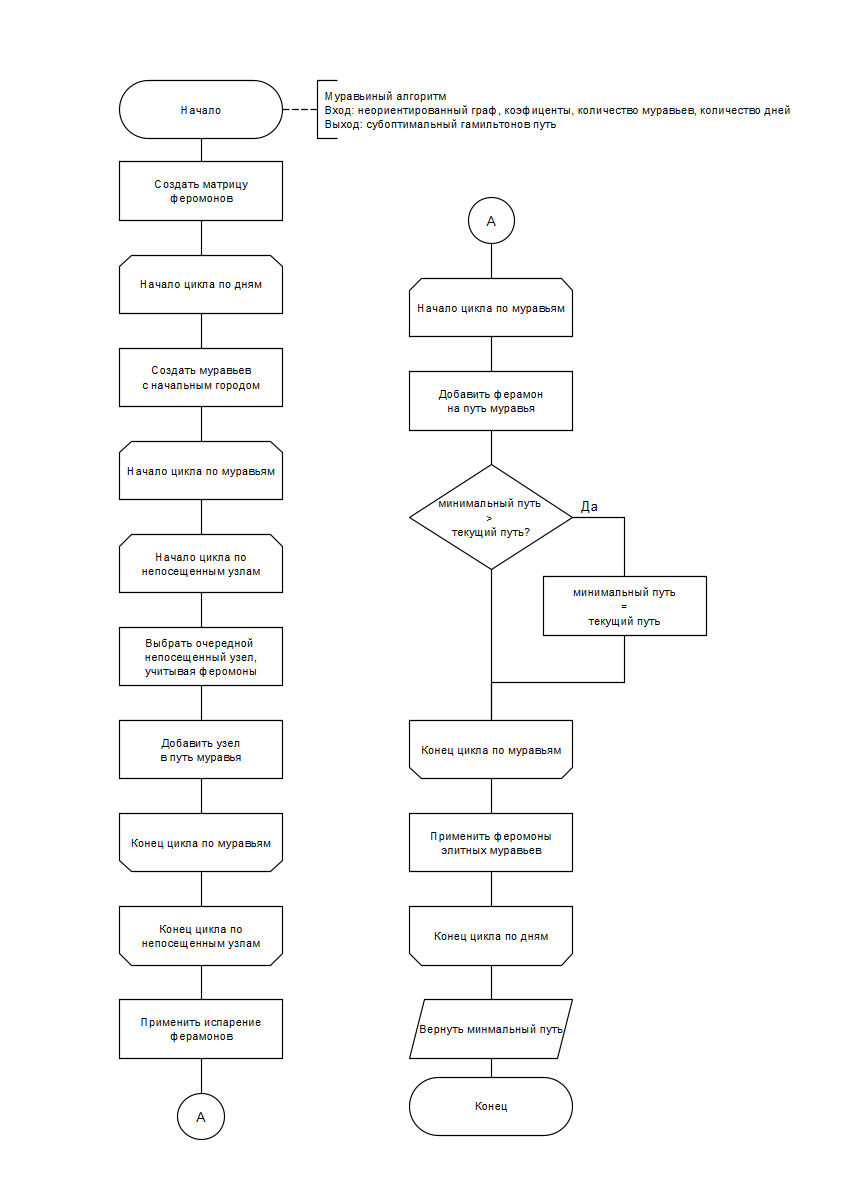
\includegraphics[width=1\textwidth]{images/schemes/ant.png}
    \caption{Схема муравьиного алгоритма}
    \label{fig:ant}
\end{figure}

\clearpage

\paragraph*{ВЫВОД} ${}$ \\

В результате конструкторского раздела были определены требования к программному обеспечению и приведены схемы алгоритма полного перебора и муравьиного алгоритма для решения задачи коммивояжера.
